\chapter{Design and Development of Cell Balancing Circuit}

\indent\indent In this chapter design and development of cell balancing circuit and methods followed in development and testing of  the balancing algorithm in MATLAB\textsuperscript{\textregistered} Simulink\textsuperscript{\textregistered} environment is discussed. 


\section{Cell Calancing Circuit}
As discussed in Chapter 2, switching shunt resistor method is used for the design. In which highest SOC cell is discharged through a shunt resistance and the discharging is controlled with \acrshort{mosfet} as shown in the Figure 3.1. A diode is connected in series with resistance to avoid any reverse current during charging of battery pack.

\begin{figure}[h!]
    \centering
    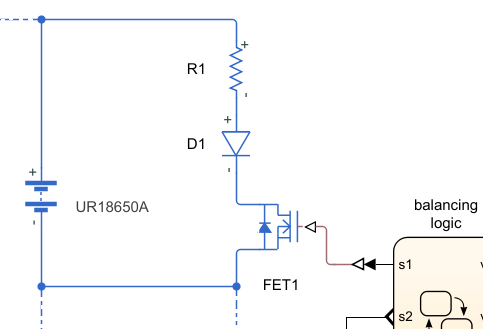
\includegraphics[]{Chapter3/Figures/cell_bal_ckt.PNG}
    \caption{Switched shunt cell balancing circuit}
\end{figure}

\subsection{Bleed Resistor}
The value of bleed resistor chosen on the basis of percentage of time the cell balancing circuit is enabled and the delta leakage current. Since this balancing circuit is meant for an \acrshort{ev} keeping power saving in mind an assumption that \acrshort{bms} will be ON for 20 percent of the time is made.

Depending on the time available for balancing and capacity of the battery pack the balancing current need to be decided. Since, BQ76PL455A \acrshort{ic} can support up to 16 Li-ion cells which is nearly 4Ah, after referring balance time versus balance current graph shown in Fig 3.2 a balancing current of 200 mA is chosen for the design. So the circuit will be able to balance the battery pack in about 10 hours in worst case i.e when the pack has some cells fully charged and some cells are near empty.

\vspace{0.5cm}

\begin{figure}[h!]
    \centering
    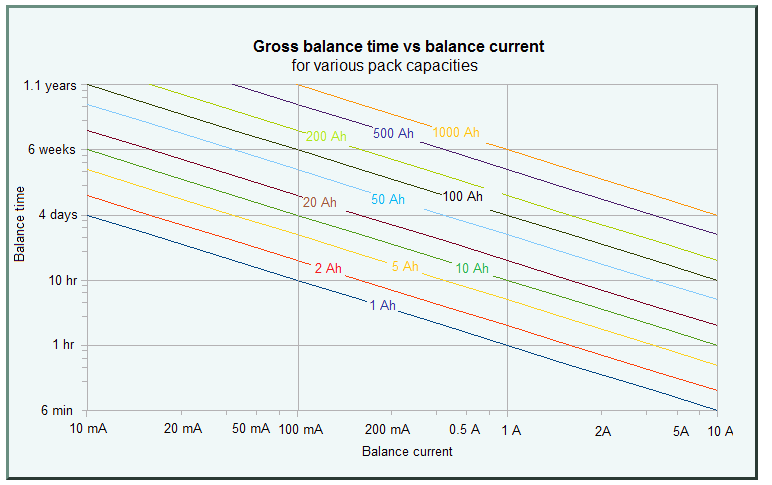
\includegraphics[scale = 0.72]{Chapter3/Figures/balcurrent_graph.PNG}
    \caption{Balancing time versus balance current graph taken from \cite{wpbalcur} }
\end{figure}

From UR18650 Li-ion cell datasheet nominal cell voltage $V = 3.7V$ and balancing current $I= 200 mA$. Using Ohm's law,

\[ V = IR\]
\[ R = \frac{V}{I}\]
\[ R = \frac{3.7}{200 *10^-^3}\]
\[ R = 18.5 \Omega\]

\subsection{Schematic of cell balancing circuit}
A MATLAB\textsuperscript{\textregistered}-Simulink\textsuperscript{\textregistered} model is developed for a battery containing 3 cells. For each cell a parallel balancing path is provided and a \acrshort{mosfet} is used to control cell discharging for balancing purpose. The state of each \acrshort{mosfet} in the design depends on the balancing logic block output as shown in Figure 3.3.

\begin{figure}[h!]
    \centering
    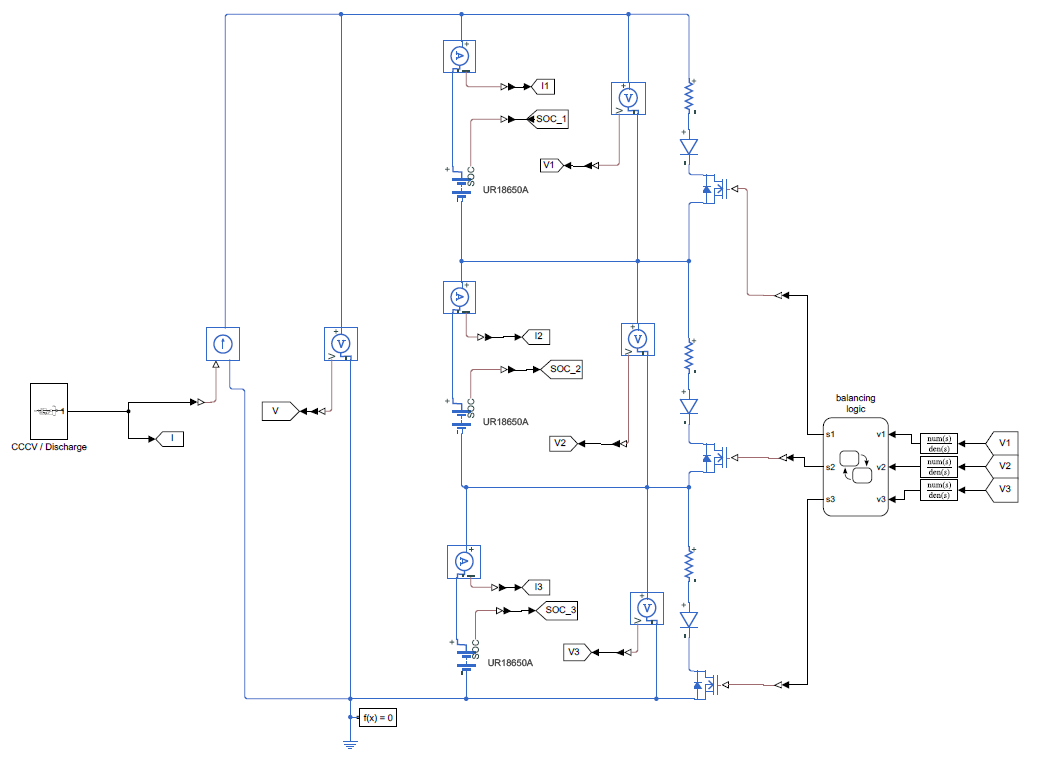
\includegraphics[scale = 0.6]{Chapter3/Figures/mainmodel.PNG}
    \caption{MATLAB\textsuperscript{\textregistered}-Simulink\textsuperscript{\textregistered} model to simulate passive cell balancing}
\end{figure}

\subsection{Simscape™}
Simscape™ is physical modelling add-on for Simulink\textsuperscript{\textregistered} environment. It provides battery cell models with other physical components like diode,resistor etc. which are designed by application engineers using physical data sets, so these models are very close to real hardware and gives good simulation results.

Panasonic UR18650 Li-ion cell model from Simscape™ Library is used for Simulink\textsuperscript{\textregistered} model. The cell model works based on look-up tables and user has freedom to override parameters like initial SOC level of cells, cell voltages etc as shown in figure 3.4.

\begin{figure}[h!]
    \centering
    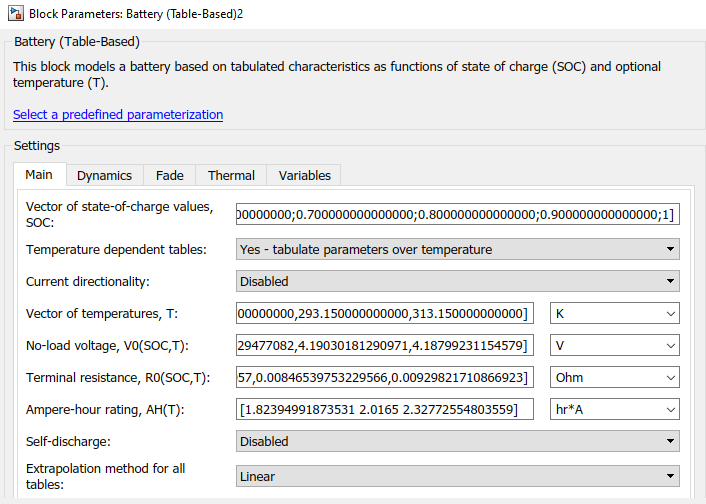
\includegraphics[scale = 0.72]{Chapter3/Figures/battery_model.PNG}
    \caption{Look up table of Simscape™ UR18650 cell model }
\end{figure}

\section{Cell balancing algorithm }
\subsection{Balancing Logic}
To perform passive cell balancing individual cell voltages or SOCs are sampled to decide which cell has to discharged via bleed resistor. The algorithm uses cell voltages to make decisions since it is easy to measure cell voltages rather then estimating individual cell's state of charge. When difference of minimum and maximum cell voltage becomes greater than 0.01V the battery pack is said to be imbalanced and it is left to the designer to choose this voltage difference value depending on extent of balancing required. The Figure 3.5 shows flowchart representation of the algorithm.

\begin{figure}[H]
    \centering
    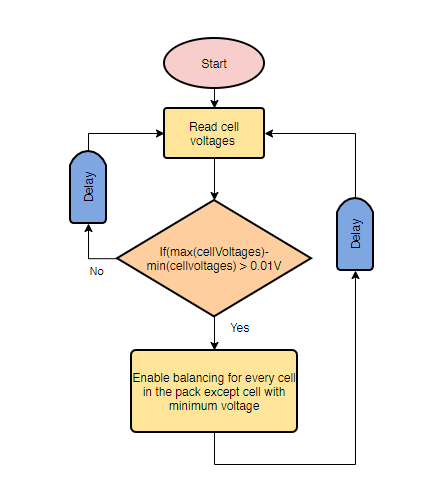
\includegraphics[]{Chapter3/Figures/logic.PNG}
    \caption{Balancing Logic flowchart}
\end{figure}

\subsection{Stateflow\textsuperscript{\textregistered}}
Stateflow\textsuperscript{\textregistered} is logic tool used to model systems using state machines and flow charts in Simulink\textsuperscript{\textregistered} environment. During simulations state switching can be visualised and debugging is made easy so that potential bugs are eliminated in early stages. Using Hardware Support packages code can be generated using Embedded code generator and it also provides options to generate code which is compliant with industry standards.



\begin{figure}[H]
    \centering
    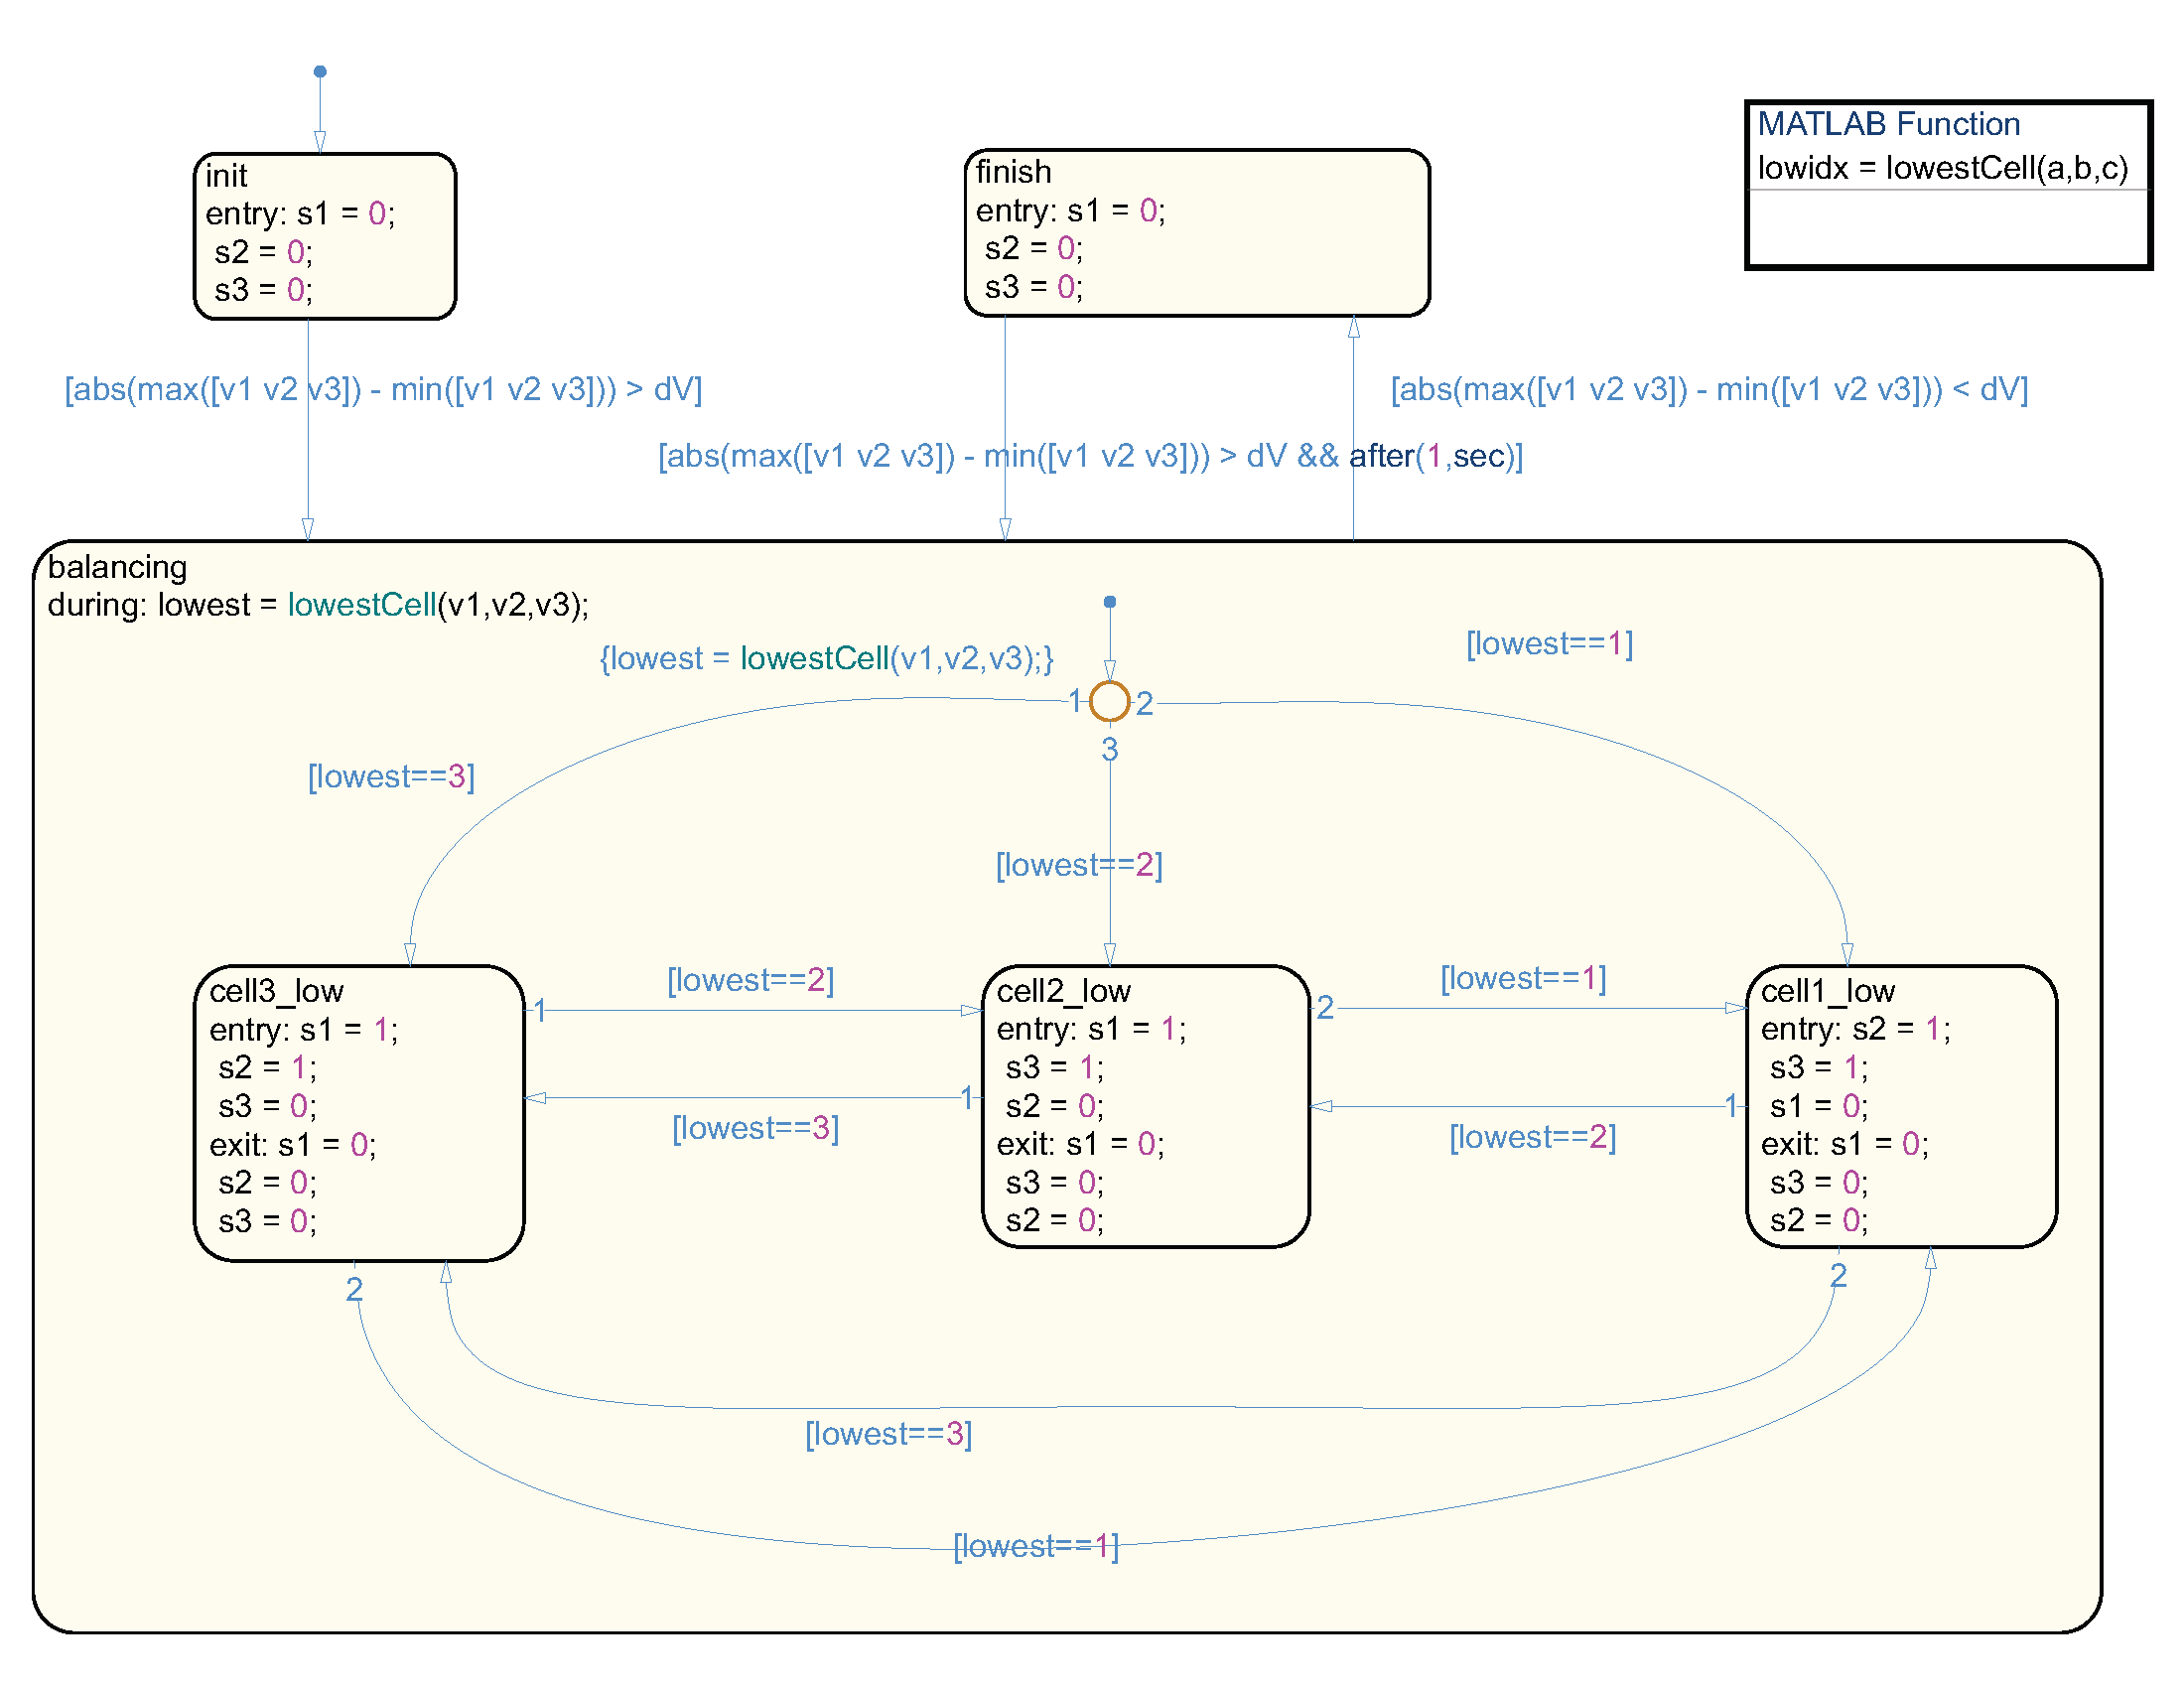
\includegraphics[scale = 0.6]{Chapter3/Figures/balancing logic.png}
    \caption{State machine for cell balancing in Stateflow\textsuperscript{\textregistered}}
\end{figure}


The logic represented in flowchart is reproduced in Stateflow\textsuperscript{\textregistered} as a state machine. The Stateflow\textsuperscript{\textregistered} diagram of the balancing logic is shown in Figure 3.6.

\vspace{1cm}

In this chapter, the details of design and development of cell balancing circuit and simulation of balancing algorithm in Simulink\textsuperscript{\textregistered}-Matlab\textsuperscript{\textregistered} is discussed. The results obtained during simulation validates the balancing algorithm. In the next chapter, implementation of balancing circuit on printed circuit board is discussed.